\chapter{Software základní desky}
Tato kapitola se zaměřuje na software základní desky ProtoPlantu a detailně popisuje jeho funkci.
Na software ostatních modulů se zaměřuje následující kapitola \ref{chap:moduleSoftware}.

\paragraph{Blokové schéma funkce softwaru základní desky}
Schéma funkce softwaru základní desky je shrnuto blokovým diagramem XXX.

\section{Sdílené knihovny}
Z~důvodu usnadnění programování základní desky i ostatních rozšiřujících modulů jsem vytvořil několik sdílených knihoven. 
V~nich je zahrnuto:
\begin{itemize}
    \item konfigurace systému
    \item nastavení jednotlivých pinů dle standardního rozložení, vč. možnosti nastavení vlastního
    \item práce s~displayem
    \item práce s~tlačítky
    \item řízení H-můstků
    \item ovládání senzorů
\end{itemize}
Díky těmto knihovnám je většina zdrojového kódu uložena v~nich. 
Koncový uživatel, který se rozhodne software modifikovat, poté pouze v~hlavním programu definuje, které moduly spustit a do konfiguračního souboru zapíše nastavení daných modulů.


\paragraph{Konfigurace softwaru}
Celý software 

\section{Datové sběrnice}
ProtoPlant primárně využívá dvě datové sběrnice:
\begin{itemize}
    \item I\superscript{2}C
    \item OneWire
\end{itemize}

\paragraph{Sběrnice I\superscript{2}C}
Tuto sběrnici používá ProtoPlant pro komunikaci se zařízeními na stejné desce, případně pro řízení LCD displeje instalovaného na řídícím panelu (připojení přes PanCon). 

\subparagraph{Princip}
Na sběrnici je připojeno jedno zařízení jakožto master (řídící) a jedno, či více zařízení jako slave (řízená).
Tato zařízení jsou navzájem propojena dvěma dráty (proto se I\superscript{2}C někdy přezdívá TwoWire), serial clock (SCL) a serial data (SDA).
Každé ze slave zařízení má sedmibitovou adresu (např. 0xE0), která musí být pro každé zařízení na jedné sběrnici odlišná.
Některá zařízení mají tuto adresu pevně zapsanou a nelze ji měnit, zatímco u~jiných ji lze změnit.
Zařízení připojené jako v~režimu master tuto adresu nepotřebuje, vzhledem k~tomu, že on sám vždy adresuje jen jedno ze zařízení.

\subparagraph{Komunikační protokol}
Za klidového stavu (neprobíhá žádná komunikace) jsou obě linky (SDA i SCL) připojeny nastaveny na HIGH.
Jakmile chce master zahájit komunikaci, vyšle takzvaný startovní signál, po kterém následuje adresa daného zařízení, jejíž nultý bit určí, zda chce master číst, nebo zapisovat.
Dále následují datové bity.
Jakmile jsou všechna data přenesena, vyšle master stop signál, čímž ukončí komunikaci a sběrnice se vrátí do klidu.
Rychlost celého přenosu určuje pulsování linky CLK.
Celý proces názorně zobrazuje obrázek \ref{fig:I2C-protocol}.

\begin{figure}[h]
   \centering
   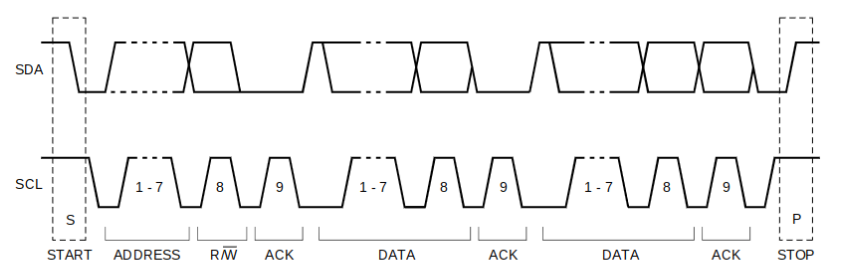
\includegraphics[width=\textwidth]{img/I2C.png}
   \caption{Celý datový přenos po I2C sběrnici.}
   \label{fig:I2C-protocol}
\end{figure}

\paragraph{Sběrnice OneWire}
Sběrnici OneWire používá ProtoPlant pro komunikaci s teplotními čidly DS18B20. 

\section{Komunikace mezi jednotlivými moduly}

\section{Bezdrátová komunikace}

\chapter{Software dalších modulů}
\label{chap:moduleSoftware}

\chapter{Zvláštní stavy}

\paragraph{Nouzový režim}
\label{paragraph:nouzovyRezim}


\newpage